% Metodologia 3-4 pags, desenho da pesquisa (BPMN, fases e atividades, exemplos nos tcs)
% Cronograma - datas, quando vai ser feito, desde o inicio do projeto la no anteprojeto, proposta, o que foi feito em MPA, o que foi tento entre um semestre e outro, o que ficou de resultado para o TC1
%==============================================================================
\chapter{METHODOLOGY}\label{methodology}
%==============================================================================

% Neste capitulo sera apresentado a metodologia, técnicas e procedimentos que foram utilizadados no decorrer deste estudo. Comecando com a \Cref{sec:met-intro}, onde é apresentada o significado de pesquisa. Na \Cref{sec:met-classification}, será feita a classificação da pesquisa utilizando termos e definições apresentados por \cite{Prodanov:2013}. Em seguida na \Cref{sec:met-design}, é apresentado como este estudo foi conduzido, junto com o desenho de pesquisa, o cronograma da pesquisa, com datas limites e espaços de tempo se encontra na \Cref{sec:met-schedule}.

In this chapter, we presente the methodology, techniques and procedures that were used in the course of this study. 
Starting with \Cref{sec:met-intro}, where we presente the context of the research. 
In \Cref{sec:met-classification}, the search will be classified using terms and definitions presented by \textcite{Prodanov:2013}. 
Then in \Cref{sec:met-design}, it is presented how this study was conducted, along with the research design, the research schedule, with deadlines and time spaces is in \Cref{sec:met-schedule}.

\section{Introduction}\label{sec:met-intro}

% Para que em um estudo os objetivos sejam alcançados com sucesso, a pesquisa cientifica é considerada muito importante pelas suas contribuições. De acordo com \cite{pingping_yulan_2013}, o objetivo de uma pesquisa é explorar a presente situação e o desenvolvimento do mundo, sob os objetivos estabelecidos anteriormente e planos de conhecimento desconhecidos.

In order for the objectives of a study to be successfully achieved, scientific research is considered very important for its contributions. 
According to \cite{pingping_yulan_2013}, the purpose of a research is to explore the present situation and development of the world, under the previously set goals and unknown knowledge plans.

% Existem diversas maneiras com que a pesquisa cientifica pode ser conduzida e é designado aos pesquisadores definirem qual utilizar, visando a maior relevância nos seus resultados. É de muita importância que sejam escolhidos como base para o desenvolvimento da pesquisa, autores e estudos de sucesso, pois como \cite{dampier_wilson} diz, "O método científico é um processo através do qual cada avanço para o estado da arte é construído sobre verdades conhecidas e avanços anteriores".

There are several ways in which scientific research can be conducted and it is assigned to researchers to define which one to use, aiming at the greatest relevance in their results. 
It is very important that they are chosen as the basis for the development of research, authors and successful studies, because as \textcite{dampier_wilson} says, the advances made previously and the known truths, serve as a basis for the advances of the scientific method.


\section{Research Classification}\label{sec:met-classification}

% A classificação desta pesquisa se deu de acordo com as definições feitas por \cite{Prodanov:2013}, na \Cref{fig:research-classification} a classificação da pesquisa esta separada por quatro grupos, cada um com suas respectivas categorias, são os grupos: 
% \begin{inparaenum}[(1)]
%   \item According to the Approach;
%   \item According to the Nature;
%   \item According to the Objectives;
%   \item According to the Procedures.
% \end{inparaenum}
% Na imagem os retangulos preenchidos com cor azul representam os que se aplicam a presente pesquisa. 

The classification of this research was given according to the definitions made by \textcite{Prodanov:2013}, in \Cref{fig:research-classification} the classification of the research is separated by four groups, each with its respective categories, are the groups: 
\begin{inparaenum}[(i)]
  \item According to the \textbf{Approach};
  \item According to the \textbf{Nature};
  \item According to the \textbf{Objectives};
  \item According to the \textbf{Procedures}.
\end{inparaenum}
In \Cref{fig:research-classification} the rectangles filled with blue color represent those that apply to this research. 

% Iniciando com o ponto de vista da natureza, esta se encaixa em \textbf{Applied Research}, pois busca aplicar novos conhecimentos gerados em problemas objetivos, envolvendo verdades, interesses e demandas locais. Trazendo para a realidade deste trabalho, os conhecimentos gerados se refere a todos os dados levantados relacionados a extensão no decorrer do estudo, e o problema objetivo é a burocracia envolvida nos projetos de extensão.

Starting with the point of view of nature, this fits into \textbf{Applied Research}, as it seeks to apply new knowledge generated in objective problems, involving truths, interests and local demands. 
Bringing to the reality of this work, the knowledge generated refers to all the data collected related to outreach in the course of the study, and the objective problem is the bureaucracy involved in \acp{OA}.

% Tendo em vista os objetivos, esta é classificada como \textbf{Exploratory Research} pois para alcancar os objetivos definidos, pesquisas na literatura cinza e questionários com pessoas relacionadas ao assunto, foram executados. Sendo assim, utilizando o que ja existe como base, busca-se construir uma nova solução aprimorada.

In view of the objectives, this is classified as \textbf{Exploratory Research} because to achieve the defined objectives, research in the grey literature and questionnaires with people related to the subject were performed. 
Thus, using what already exists as a basis, we seek to build a new improved solution.

% Em relação aos procedimentos técnicos, se aplica \textbf{Case Study}, pois busca coletar informações de individuos, ferramentas, processos, relacionados com o tema principal utilizando métodos \textbf{Qualitatives}, para ser possível colocar os resultados e gráficos e analisa-los, and \textbf{Quantitavive}, permitindo o entendimento mais profundo do que foi respondido. A classificação \textbf{Survey} também se aplica, por ser esta uma das maneiras de coleta de informação utilizada pelos pesquisadores, antes da execução com o público respondente, um teste piloto foi conduzido, para validar organização, completude, coerência e outros pontos do questionário, mais deste será discutido na \Cref{sec:5}.

In relation to technical procedures, \textbf{Case Study} is applied, as it seeks to collect information from individuals, tools, processes, related to the main theme using \textbf{Qualitative} methods, to be able to place the results and graphs and analyze them, and \textbf{Quantitavive}, allowing a deeper understanding of what was answered. 
The \textbf{Survey} classification also applies, as this is one of the ways of collecting information used by researchers. 
Before the survey execution with the participants, a pilot test was conducted to validate organization, completeness, coherence and other points of the questionnaire, more of this will be discussed in \Cref{sec:5}.

% Por último, o trabalho também se encontra classificado como \textbf{Documentrary Research}, por usar como base de conhecimento, materiais que ainda não receberam um tratamento analítico, como resultados de pesquisas na internet, o assunto sobre literatura cinza sera explicado melhor na \Cref{sec:4}.

Finally, the study is also classified as \textbf{Documentary Research}, for using as a knowledge base, materials that have not yet received an analytical treatment, such as internet search results, the subject of grey literature will be better explained in \Cref{grey_literature}.

\begin{figure}[!htb]
  \caption{Research Classification}
  \label{fig:research-classification}
  \begin{center}
    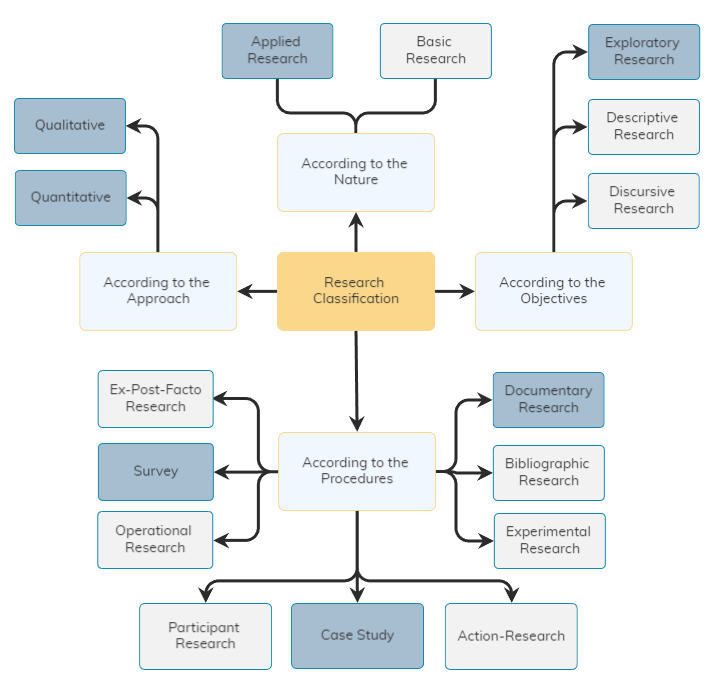
\includegraphics[width=14cm]{img/2-pesquisa-survey.png}
  \end{center}
  \fonte{Adapted from \cite{Prodanov:2013}.}
\end{figure}

\section{Research Design}\label{sec:met-design}

% Na \Cref{fig:research-design} está representada o fluxograma seguido no decorrer desta pesquisa, as atividades nele posicionadas estão divididas entre cinco fases:
In \Cref{fig:research-design} is represented the flowchart followed in the course of this research, the activities placed in it are divided into five phases:
\begin{inparaenum}[(1)]
  \item Information gathering;
  \item Partial development;
  \item Development;
  \item Evaluation;
  \item Publish.
\end{inparaenum}

% A primeira fase, \textbf{Information gathering}, é focada em organizar estruturas de pesquisa, questionarios, priorização de informações, aprendizado sobre o tema da pesquisa. Principalmente direcionada a produzir dois importantes artefatos da pesquisa, a revisão na literatura cinza e o survey com possíveis usuários finais.

The first phase, \textbf{Information Gathering}, is focused on organizing research structures, questionnaires, prioritization of information, and learning about the research topic. Mainly aimed at producing two important artifacts of the research, the review in the grey literature and the survey with possible end users.

% Seguindo para a segunda fase, \textbf{Partial Development}, onde foi decidido entre os envolvidos no projeto, que não seria viável implementar todo a ferramenta neste primeiro momento, então apenas algumas funcionalidades mais importantes e que ja seriam suficientes para um produto em estado inicial, seriam desenvolvidas.
% Dentro da fase de \textbf{Publish}, os dois Term Papers serão escritos e defendidos, ocorrendo de forma paralela ao desenvolvimento da ferramenta, majoritariamente acontecendo na fase de \textbf{Development}.

Moving on to the second phase, \textbf{Partial Development}, where it was decided among those involved in the project, that it would not be feasible to implement the entire tool at this first moment, so only some more important functionalities and that would already be sufficient for a \ac{MVP}, which is defined by \textcite{ries2011lean} as a new product version that enables a team to gather the most verified customer learning possible with the least amount of work, would be developed.
Within the \textbf{Publish} phase, the two \acp{TP} will be written and defended, occurring in parallel to the development of the tool, mostly happening in the \textbf{Development} phase.

% Após ja existir uma versão estável da ferramenta, onde usuários possam utiliza-la, esta será disponível para uso real, permitindo que um curso de extensão da Unipampa seja cadastrado e abrindo vagas para inscrições de participantes, com isto na fase de \textbf{Evaluation}, serão coletados os feedbacks, analisado os resultados e melhorias na ferramenta serão feitas.

After there is a stable version of the tool, where users can use it, it will be available for real use, allowing UNIPAMPA's outreach activities to be registered and opening vacancies for participant or volunteer registrations, with this in the phase of \textbf{Evaluation}, feedbacks will be collected, analyzed the results and improvements in the tool will be made.

\begin{figure}[htb]
  \caption{Research Design}\label{fig:research-design}
  \begin{center}
    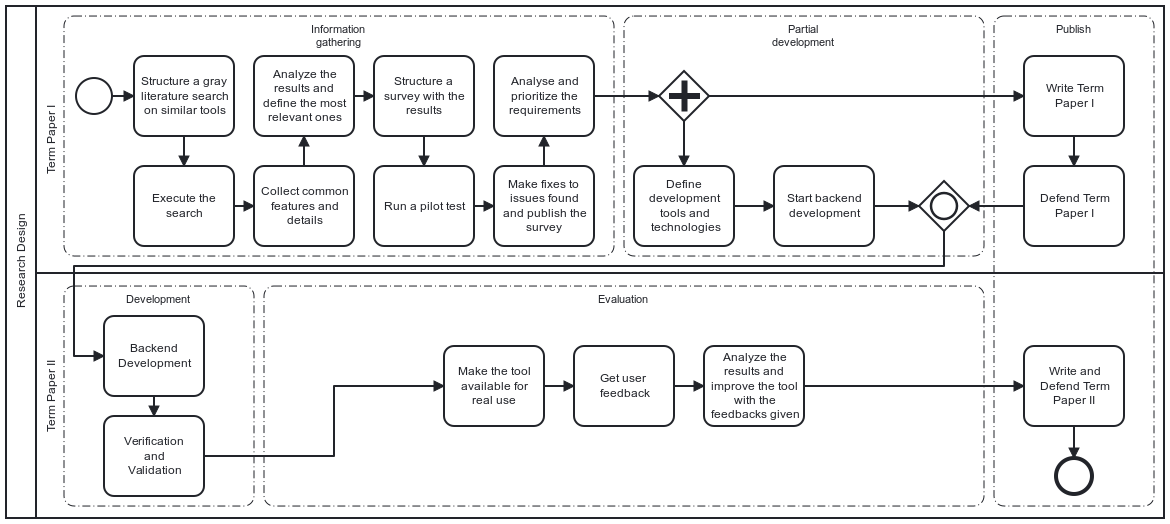
\includegraphics[width=16cm]{img/2-research-diagram.png}
  \end{center}
  \fonte{Author.}
\end{figure}

\section{Research Schedule}\label{sec:met-schedule}

% Para facilitar a visualização de como as atividades se deram ao decorrer do tempo, na \Cref{tbl:schedule} é apresentado todo o cronograma do que foi planejado desde o levantamento de informações até a defesa do Term Paper II.

To facilitate the visualization of how the activities took place over time. 
\Cref{tbl:schedule} presents the entire schedule of what was planned from the collection of information to the defense of \acl{TP} II.

\begin{table}[!htb]
  \centering
  \caption{Research Schedule}
  \label{tbl:schedule}
  \scriptsize
  \begin{tabular}{p{4cm}|l|lllll|lll}
    \bottomrule
    \rowcolor[rgb]{0.753,0.753,0.753} \multicolumn{1}{c|}{{\cellcolor[rgb]{0.753,0.753,0.753}}}                                       & \multicolumn{1}{c|}{\textbf{2021/2}} & \multicolumn{5}{c|}{\textbf{2022/1}} & \multicolumn{3}{c|}{\textbf{2022/2}}                                                                                                                                                                                                                                           \\
    \hhline{>{\arrayrulecolor[rgb]{0.753,0.753,0.753}}->{\arrayrulecolor{black}}---------|}
    \rowcolor[rgb]{0.753,0.753,0.753} \multicolumn{1}{c|}{\multirow{-2}{*}{{\cellcolor[rgb]{0.753,0.753,0.753}}\textbf{ Activities}}} & \textbf{Nov - Mar}                   & \multicolumn{1}{c}{\textbf{Apr}}     & \textbf{May}                         & \textbf{Jun}                         & \multicolumn{1}{l}{\textbf{Jul}}     & \textbf{Aug}                         & \textbf{Sep Oct Nov}                 & \textbf{Dec}                         & \multicolumn{1}{c|}{\textbf{Jan}}    \\
    \hline
    \rowcolor[rgb]{0.914,0.914,0.914} Plan and execute systematic review in the grey literature                                       & {\cellcolor[rgb]{0.753,0.753,0.753}} &                                      &                                      &                                      &                                      &                                      &                                      &                                      &                                      \\
    Plan and execute survey with target users                                                                                         &                                      & {\cellcolor[rgb]{0.753,0.753,0.753}} &                                      &                                      &                                      &                                      &                                      &                                      &                                      \\
    \rowcolor[rgb]{0.914,0.914,0.914} Analyze results from previous steps and map requirements                                        &                                      & {\cellcolor[rgb]{0.753,0.753,0.753}} & {\cellcolor[rgb]{0.753,0.753,0.753}} &                                      &                                      &                                      &                                      &                                      &                                      \\
    Plan and start tool development                                                                                                   &                                      &                                      & {\cellcolor[rgb]{0.753,0.753,0.753}} & {\cellcolor[rgb]{0.753,0.753,0.753}} &                                      &                                      &                                      &                                      &                                      \\
    \rowcolor[rgb]{0.914,0.914,0.914} Write Term Paper I                                                                              &                                      &                                      &                                      & {\cellcolor[rgb]{0.753,0.753,0.753}} & {\cellcolor[rgb]{0.753,0.753,0.753}} & {\cellcolor[rgb]{0.753,0.753,0.753}} &                                      &                                      &                                      \\
    Defend Term Paper I                                                                                                               &                                      &                                      &                                      &                                      &                                      & {\cellcolor[rgb]{0.753,0.753,0.753}} &                                      &                                      &                                      \\
    \rowcolor[rgb]{0.914,0.914,0.914} Continue the development of the tool                                                            &                                      &                                      &                                      &                                      &                                      & {\cellcolor[rgb]{0.753,0.753,0.753}} & {\cellcolor[rgb]{0.753,0.753,0.753}} & {\cellcolor[rgb]{0.753,0.753,0.753}} &                                      \\
    Execute a real use case on the tool                                                                                               &                                      &                                      &                                      &                                      &                                      &                                      &                                      & {\cellcolor[rgb]{0.753,0.753,0.753}} &                                      \\
    \rowcolor[rgb]{0.914,0.914,0.914} Write Term Paper II                                                                             &                                      &                                      &                                      &                                      &                                      &                                      &                                      & {\cellcolor[rgb]{0.753,0.753,0.753}} & {\cellcolor[rgb]{0.753,0.753,0.753}} \\
    Defend Term Paper II                                                                                                              &                                      &                                      &                                      &                                      &                                      &                                      &                                      &                                      & {\cellcolor[rgb]{0.753,0.753,0.753}} \\
    \toprule
  \end{tabular}
  \fonte{Author.}
\end{table}


\section{Chapter Summary}\label{sec:met-summary}

% Neste capitulo foi apresentado o significado de metodologia, e como ela pode ser classificada dentro de um ambito cientifico, juntamente com quais termos que se aplicam ao presente Term Paper. Além disso foi apresentado o design de pesquisa contendo os passos realizados pelo autor, como também os que serão dados.

In this chapter we have presented the meaning of methodology, and how it can be classified within a scientific scope, along with what terms apply to this \ac{TP}. 
In addition, the research design was presented containing the steps taken by the author, as well as those that will be given.

%------------------------------------------------------------------------------

%------------------------------------------------------------------------------
% Migrar o anteprojeto
%  Falar sobre a literatura cinza para identificar as ferramentas, atualizar a figura
%  Atualizara imagem colocar o survey e na classificaç~ao de pesquisa adicionar o survey. Retirar pesquisa documental
%  Olhar os outros TCCs para exemplo
%  Detalhar mais o que é cada caixa do desenho de pesquisa
%  Detalhar mais cada caixinha da figura 3
% Imagens: Cronograma desde 2021/2, atualizar (segundo semestre vai ate julho) (prox ano comeca em julho e vai ate janeiro) 
